\documentclass[12pt,oneside]{report}

\usepackage[utf8]{inputenc}
\usepackage[T1]{fontenc}
\usepackage{geometry}
\geometry{a4paper, margin=1in}

\usepackage{graphicx}
\usepackage{tikz} % Used for generating a standalone placeholder figure
\usepackage{hyperref}

% Hyperlink configuration
\hypersetup{
  colorlinks = true,
  urlcolor   = blue,
  linkcolor  = blue,
  citecolor  = red
}

% Define a custom command for keywords
\newcommand{\keywords}[1]{\textbf{Keywords:} #1}

% Project Information
\title{\textbf{Title of Your Degree Project}}
\author{Author1 Name, Author2 Name, Author3 Name, and Author4 Name}
\date{\today}

\begin{document}

%%%%%%%%%%%%%%%%%%%%%%%%%%%%%%%%%%%%%%%%%%%%%%%%%%%%%%%%%%%%%%%%%%%%%%%%%%%%%%%%%%%%%%%%%%%%%%%%
% Front Matter
%%%%%%%%%%%%%%%%%%%%%%%%%%%%%%%%%%%%%%%%%%%%%%%%%%%%%%%%%%%%%%%%%%%%%%%%%%%%%%%%%%%%%%%%%%%%%%%%
\pagenumbering{roman}

% Cover page
\maketitle
\thispagestyle{empty}
\newpage

% Acknowledgments
\chapter*{Acknowledgments}
\addcontentsline{toc}{chapter}{Acknowledgments}
Expressing gratitude is always good practice.

% Abstract
\chapter*{Abstract}
\addcontentsline{toc}{chapter}{Abstract}
The abstract (200--500 words) should provide a comprehensive overview of the entire
project, clearly stating the formalisms, techniques, tools, and languages
used. It should not be limited to describing the problem addressed, but must also describe
the proposed solution alongside its evaluation. It must not include bibliographic
references or citations to other parts of the report, nor should it use
acronyms without defining their meaning first.

\vspace{1em}
\noindent\keywords{Template, Degree Projects, Computer Science}

\newpage

% Table of Contents
\tableofcontents
\newpage

%%%%%%%%%%%%%%%%%%%%%%%%%%%%%%%%%%%%%%%%%%%%%%%%%%%%%%%%%%%%%%%%%%%%%%%%%%%%%%%%%%%%%%%%%%%%%%%%
% Main Matter
%%%%%%%%%%%%%%%%%%%%%%%%%%%%%%%%%%%%%%%%%%%%%%%%%%%%%%%%%%%%%%%%%%%%%%%%%%%%%%%%%%%%%%%%%%%%%%%%
\pagenumbering{arabic}

% Introduction
\chapter{Introduction}

This chapter provides the motivation for the work, states and defines the problem, clearly sets the objectives (the general goal of the project, if applicable or if embedded within a larger initiative, and the specific objectives), presents the expected results, summarizes the main conclusions, and outlines the overall organization of the document.

This and the following chapters may include references. Examples of citations include \cite{CitekeyArticle}, \cite{CitekeyBook}, \cite{CitekeyInproceedings}, \cite{CitekeyManual}, and \cite{CitekeyMisc}.

%%%%%%%%%%%%%%%%%%%%%%%%%%%%%%%%%%%%%%%%%%%%%%%%%%%%%%%%%%%%%%%%%%%%%%%%%%%%%%%%%%%%%%%%%%%%%%%%

% Literature Review
\chapter{Literature Review}

A review of background work (products, processes, publications, etc., at both academic and commercial levels) related to the topic of this project. It may also include (if necessary) a brief introduction to fundamental concepts required to understand the work.

\section{First Section}
Chapters can include sections such as this one, which can also cross-reference other sections, such as Section~\ref{sec:second}.

\section{Second Section}\label{sec:second}
This section also includes a subsection.

\subsection{The Subsection}
This is the subsection.

%%%%%%%%%%%%%%%%%%%%%%%%%%%%%%%%%%%%%%%%%%%%%%%%%%%%%%%%%%%%%%%%%%%%%%%%%%%%%%%%%%%%%%%%%%%%%%%%

% Core Contribution
\chapter{Core Contribution}
The core chapter covers the original contribution and main engineering output of the degree project, including key decisions made along the way. For example, it may cover requirements, analysis, and solution design. If the project includes an implementation, it should be described in terms of architectural and design decisions. Low-level programming details should be reserved for the appendices.

Figures and tables can be embedded in the document, and both must be referenced directly in the text. For instance, Figure~\ref{fig:logos} shows a placeholder diagram, while Table~\ref{table:data} contains sample numbers.

\begin{figure}[htbp]
  \centering
  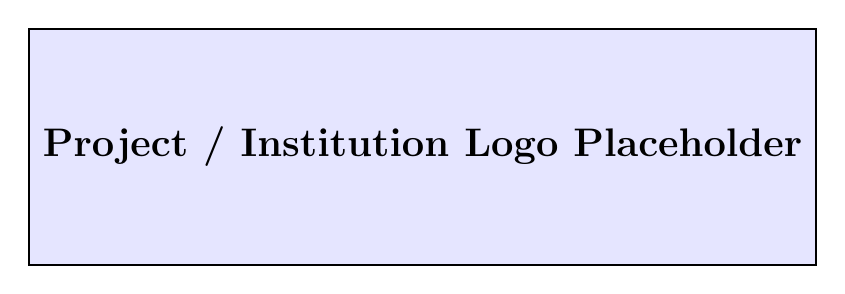
\begin{tikzpicture}
    \draw[thick, fill=blue!10] (0,0) rectangle (10,3);
    \node at (5,1.5) {\Large \textbf{Project / Institution Logo Placeholder}};
  \end{tikzpicture}
  \caption{Standalone vector placeholder for institutional logos}
  \label{fig:logos}
\end{figure}

\begin{table}[htbp]
\centering
\begin{tabular}{| c | c | c | c |} 
  \hline
  Col1 & Col2 & Col3 & Col4 \\  
  \hline
  1 & 970 & 67 & 941 \\ 
  2 & 668 & 845 & 141 \\
  3 & 800 & 383 & 464 \\
  4 & 143 & 683 & 502 \\
  \hline
\end{tabular}
\caption{Table with data}
\label{table:data}
\end{table}

%%%%%%%%%%%%%%%%%%%%%%%%%%%%%%%%%%%%%%%%%%%%%%%%%%%%%%%%%%%%%%%%%%%%%%%%%%%%%%%%%%%%%%%%%%%%%%%%

% Experimental Evaluation
\chapter{Experimental Evaluation}
It may be necessary to include an Experimental Evaluation chapter, detailing tests performed (test cases), results obtained, and a corresponding discussion, which may include comparative analysis.

%%%%%%%%%%%%%%%%%%%%%%%%%%%%%%%%%%%%%%%%%%%%%%%%%%%%%%%%%%%%%%%%%%%%%%%%%%%%%%%%%%%%%%%%%%%%%%%%

% Conclusions
\chapter{Conclusions and Future Work}
This chapter evaluates the achievements and obstacles encountered, comparing what was originally planned against what was actually accomplished. It highlights the main contributions, discusses potential extensions of the work, and presents a self-critique regarding what was done and what remains missing.

%%%%%%%%%%%%%%%%%%%%%%%%%%%%%%%%%%%%%%%%%%%%%%%%%%%%%%%%%%%%%%%%%%%%%%%%%%%%%%%%%%%%%%%%%%%%%%%%
% Back Matter
%%%%%%%%%%%%%%%%%%%%%%%%%%%%%%%%%%%%%%%%%%%%%%%%%%%%%%%%%%%%%%%%%%%%%%%%%%%%%%%%%%%%%%%%%%%%%%%%

% Inline Bibliography (replaces external .bib file)
\begin{thebibliography}{99}
\addcontentsline{toc}{chapter}{Bibliography}

\bibitem{CitekeyArticle}
Author, A. (2024). Title of the journal article. \emph{Journal Name}, 10(2), 123--130.

\bibitem{CitekeyBook}
Author, B., \& Coauthor, C. (2023). \emph{Title of the Book}. Publisher Name.

\bibitem{CitekeyInproceedings}
Author, D. (2022). Title of the conference paper. In \emph{Proceedings of the International Conference} (pp. 45--52).

\bibitem{CitekeyManual}
Organization. (2021). \emph{Software Reference Manual} (v2.0).

\bibitem{CitekeyMisc}
Author, E. (2025). Title of online resource or technical report. Retrieved from \url{https://example.com}

\end{thebibliography}

%%%%%%%%%%%%%%%%%%%%%%%%%%%%%%%%%%%%%%%%%%%%%%%%%%%%%%%%%%%%%%%%%%%%%%%%%%%%%%%%%%%%%%%%%%%%%%%%

% Appendices
\appendix

\chapter{Appendix 1}
Appendices contain supplementary material that is useful but not strictly essential to understanding the core report. For example, detailed technical specifications, background material, or complete source code summaries that were condensed in the main body. For software development projects, a user manual should be included here.

\section{Appendix Section}
Appendices can also be divided into sections.

\end{document}
